% THIS DOCUMENT IS FOLLOWS THE VOLERE TEMPLATE BY Suzanne Robertson and James Robertson
% ONLY THE SECTION HEADINGS ARE PROVIDED
%
% Initial draft from https://github.com/Dieblich/volere
%
% Risks are removed because they are covered by the Hazard Analysis
\documentclass[12pt]{article}

\usepackage{booktabs}
\usepackage{tabularx}
\usepackage{graphicx}
\usepackage{hyperref}
\usepackage{tcolorbox}
\usepackage{longtable}
\usepackage{multirow}
\usepackage{geometry}
\usepackage{array}
\usepackage[normalem]{ulem} % for strikethrough

\hypersetup{
    bookmarks=true,         % show bookmarks bar?
      colorlinks=true,      % false: boxed links; true: colored links
    linkcolor=red,          % color of internal links (change box color with linkbordercolor)
    citecolor=green,        % color of links to bibliography
    filecolor=magenta,      % color of file links
    urlcolor=cyan           % color of external links
}

\newcommand{\lips}{\textit{Insert your content here.}}

\input{../Comments}
%% Common Parts

\newcommand{\progname}{Industrial Plant Designer} % PUT YOUR PROGRAM NAME HERE
\newcommand{\authname}{Team 18, Chemware Engineering
\\ Kishor Pandya
\\ Dhrumil Pandya
\\ Madhu Sivapragasam
\\ Rasik Pokharel} % AUTHOR NAMES                  

\usepackage{hyperref}
    \hypersetup{colorlinks=true, linkcolor=blue, citecolor=blue, filecolor=blue,
                urlcolor=blue, unicode=false}
    \urlstyle{same}
                                


\begin{document}

\title{Software Requirements Specification for \progname: subtitle describing software} 
\author{\authname}
\date{\today}
	
\maketitle

~\newpage

\pagenumbering{roman}

\tableofcontents

~\newpage

\section*{Revision History}

\begin{tabularx}{\textwidth}{p{4cm}p{3cm}p{1cm}X}
\toprule {\textbf{Date}} & {\textbf{Author}} & {\textbf{Version}} & {\textbf{Notes}}\\
\midrule
September 27th 2024 & Kishor Pandya & 1.0 & Added the stakeholders section\\
September 28th 2024 & Dhrumil Pandya & 1.1 & Added all sections of Mandated Constraints\\
September 29th 2024 & Madhu Sivaprasam & 1.1 & Added purpose of the project\\
September 29th 2024 & Rasik Pokharel & 1.1 & Added relevant facts of the project\\
October 1st 2024 & Madhu Sivaprasam & 1.2 & Added scope of work section\\
October 2nd 2024 & Kishor Pandya & 1.2 & Added Functional Requirements\\
October 6th 2024 & Madhu Sivaprasam & 1.3 & Added usability/humanity and performance requirements\\
October 6th 2024 & Dhrumil Pandya & 1.4 & Added Business Data Model and Data Dictionary\\
October 6th 2024 & Rasik Pokharel & 1.4 & Added Scope of Product and Look and Feel Requirements\\
October 7th 2024 & Kishor Pandya & 1.5 & Added operational and environmental requirements\\
October 8th 2024 & Madhu Sivapragasam & 1.6 & Added user problems, costs and waiting room\\
October 9th 2024 & Dhrumil Pandya & 1.7 & Added Legal and Cultural Requirements\\
October 9th 2024 & Dhrumil Pandya & 1.8 & Added Tasks, User Documentation and Training \\
October 9th 2024 & Kishor Pandya & 1.9 & Added sections 14,19, and 26\\
October 9th 2024 & Rasik Pokharel & 1.10 & Added Security Requirements and Migration \\
October 11th 2024 & Kishor Pandya & 1.11 & Added Open Issues section and fixed some formatting issues \\
\textcolor{blue}{April 3rd 2024} & \textcolor{blue}{Madhu Sivapragasam} & \textcolor{blue}{2.0} & \textcolor{blue}{Removed unneeded requirement for rev 1}\\
\bottomrule
\end{tabularx}

~\\

~\newpage
\section{Purpose of the Project}
\subsection{User Business}

Our sponsor, Professor Vladimir Mahelec is looking to create a system that can simulate a factory plant's behaviour depending on a given set of inputs. Currently, Professor Mahelec and his team have developed a model that takes input data from a set of Excel tables and then processes the data before sending output data back. This input data represents different components of the factory, variable data within the components, connections between components, etc. Due to the complexity of the input data, various Excel tables are needed to store and organize the varying inputs properly. Unfortunately, creating and updating data in these Excel tables can be a complex and difficult task due to the complexity of the workbook. Therefore, users of the system need to have familiarity with their table conventions and that can be difficult if this service is used by external clients. Similarly updating data in the table can be time-consuming since each components need to have new data added and new connections defined which can be a slow process. 
\\\\
To solve this, our sponsor is requesting us to build a user interface that will allow a user to easily input the factory plant data. This would include a schema drawing tool that will allow a user to create a schema along with tooling to input any other data. While this service is initially intended for hydrogen plants, it should be customizable so that all types of factories can use the service. Eventually, Professor Mahelec intends to sell this service to other vendors and plant operators so that they can use it themselves to visualize and simulate factory plant data. 

\subsection{Goals of the Project}
\begin{itemize}
\item Develop a GUI that allows a user to create a factory plant schema, the data from this schema can then be sent to Professor Mahelec's model which will then produce the output which should also be displayed in the GUI
\item Develop other UI tooling that can accept inputs that may not be available in a factory schema GUI such that all other input data can also be successfully entered by the user
\item Develop a backend service and db layer that can the data from the UI inputs and send it to the processing model and then take the response from that model and send it back to the user
\item Develop a version control system such that a user can make a plant schema, save it and then recover it at a later date
\item Create documentation that allows for easy handover of the project after the project is complete so that our sponsor can take the project and use it easily themselves
\item Accomplish all of Professor Mahelec's requirements that he sets for the service so that he is satisfied with the end result of the project
\end{itemize}

\section{Stakeholders}

\subsection{Client} 
The client for this project is Dr. Vladimir Mahalec, who will serve as the primary point of contact throughout the development process.

\subsection{Customer} 
The target customers for this product are engineers across various disciplines who need to model industrial plants using nodes and edges to represent machines and material streams. These engineers will also use the software to run simulations of plant processes and obtain results for further analysis.

\subsection{Society}
The impact of this product on society can be understood through several perspectives:

\begin{itemize}
    \item \textbf{Efficiency in Industrial Operations:} By enabling engineers to model and simulate industrial plants, this software can help optimize plant efficiency, reduce resource consumption, and minimize waste. Improved operational efficiency can lower production costs and reduce the environmental footprint, benefiting both industry and society.
    
    \item \textbf{Advancement in Engineering Practices:} This product serves as a valuable tool for practicing engineers and students alike, allowing them to visualize complex systems and test different scenarios before real-world implementation. This can lead to more innovative designs, improved safety standards, and better overall outcomes in industrial engineering.
    
    \item \textbf{Educational Contribution:} Since the software will be used by Dr. Mahalec and his students, it contributes to advancing education and research in fields such as chemical and mechanical engineering. As a result, it supports the development of future engineers, enhancing their skills and preparedness for real-world challenges.
    
    \item \textbf{Sustainability and Environmental Impact:} By simulating industrial processes with a focus on optimizing energy use and reducing emissions, the software can aid industries in adopting more sustainable practices. This can have broader societal benefits by supporting efforts to combat climate change and promote environmentally responsible practices.
\end{itemize}

In summary, this product has the potential to positively affect society by improving industrial efficiency, advancing engineering education and practices, and contributing to sustainability efforts.

\subsection{Other Stakeholders} 
Other relevant stakeholders include: 
\begin{itemize} 
  % \item Developers: The team responsible for designing, implementing, and maintaining the product. 
  \item Investors: Individuals or companies who fund the construction and operation of industrial plants. They will hire engineers who may use this product to model and optimize production processes. 
  \item Supervisors and Academics: Faculty members, such as Dr. Mahalec and his post-graduate students, who will provide guidance during the development and evaluation of the product. 
\end{itemize}

\subsection{Hands-On Users of the Product} 
The hands-on users of this product include: 
\begin{itemize} 
  % \item Development Team: The team building the software, responsible for the design, coding, testing, and ongoing support. 
  \item Supervisors and Researchers: Dr. Mahalec and his post-graduate students, who will be involved in testing, providing feedback, and ensuring the product meets the necessary standards. 
  \item Engineers: The primary end users, who will use the product to model, simulate, and analyze the operations of industrial plants. 
\end{itemize}

\subsection{Personas}

\begin{itemize}
    \item \textbf{Process Engineer (Jane Smith)}
    
    \textbf{Background:} Jane is a process engineer with 5 years of experience in the energy sector, focusing on chemical processes like hydrogen production and refining. She holds a Master's degree in Chemical Engineering.
    
    \textbf{Goals:} Jane uses the software to design detailed models of industrial plants, focusing on optimizing energy efficiency. She frequently runs simulations to test different operational scenarios and identify bottlenecks in the system.
    
    \textbf{Challenges:} Jane is pressed for time and values user-friendly tools that allow her to visualize plant models quickly. She needs precise simulation results to support decision-making and regulatory compliance.
    
    \item \textbf{Mechanical Engineer (Sam Lee)}
    
    \textbf{Background:} Sam is a mechanical engineer specializing in designing and maintaining industrial equipment. He has a Bachelor’s degree in Mechanical Engineering and has worked in the field for 8 years.
    
    \textbf{Goals:} Sam uses the software to map out the physical layout of machinery and ensure that the plant model accurately reflects the equipment’s configuration and operation. He’s focused on improving the reliability of machinery and minimizing downtime.
    
    \textbf{Challenges:} Sam requires the software to integrate mechanical constraints, such as pressure and flow rates, to ensure the safety and efficiency of the modeled systems.
    
    \item \textbf{Graduate Researcher (Maria Gomez)}
    
    \textbf{Background:} Maria is a graduate student working under Dr. Mahalec, conducting research on advanced simulation techniques for industrial processes. She is pursuing a PhD in Chemical Engineering.
    
    \textbf{Goals:} Maria uses the software as part of her research to simulate theoretical plant models. She experiments with new configurations and operating conditions to evaluate their potential for energy savings and emissions reduction.
    
    \textbf{Challenges:} Maria needs advanced features that allow her to customize simulations and compare results across multiple scenarios. She values flexibility and the ability to export data for further analysis in other tools.
\end{itemize}

\subsection{Priorities Assigned to Users}
The highest priority will be given to users who have a significant stake in the success of the product. This includes Dr. Vladimir Mahalec, as the client and primary stakeholder, and his post-graduate students, who will rely on the software for research and academic purposes. Their feedback and requirements will be critical in shaping the development process and ensuring that the final product meets the intended goals.

\subsection{User Participation}
During the development phase, most user participation will come from the project developers and supervisors. The supervisors, particularly Dr. Mahalec and his post-graduate students, will play a key role in providing feedback and testing the product. Their input is crucial, as they will be the primary users during the initial stages and will help ensure that the software aligns with its intended functionality and usability goals.

\subsection{Maintenance Users and Service Technicians}
The development team will be responsible for maintaining the software until April 2025. After this period, Dr. Vladimir Mahalec will acquire the rights to the product, assuming responsibility for its ongoing maintenance and support. Any future updates, bug fixes, or enhancements will fall under his purview or that of any designated technical team.

\section{Mandated Constraints}
\subsection{Solution Constraints}
\subsubsection{Dual Database System Implementation}
\textbf{Description:} The software must implement a dual database system, consisting of separate user and system databases. The user database will store user-specific data like customized plant models, parameters, and configurations. The system database will store standard industry data, default equipment parameters, and operational constraints.\\\\
\textbf{Rationale:} The separation of user and system data has been explicitly requested by the supervisor to ensure data integrity, security, and ease of maintenance. This dual database setup allows flexible customization of plant models while maintaining the integrity of standard system data.\\\\
\textbf{Fit Criterion:} 
\begin{itemize}
  \item The system must use two distinct databases: one for system data and one for user data.
  \item User modifications must only affect the user database without altering the system database.
  \item The software shall prevent any write operations to the system database from the user interface.
\end{itemize}
\subsubsection{Web-Based Canvas Interface with Nodes and Arcs}
\textbf{Description:} The software must provide a web-based graphical user interface (GUI) that runs in a browser, featuring a canvas where users can create plant models using draggable nodes (representing equipment) and connect them with arcs (representing material or energy streams). The supervisor strongly suggested using React Flow which is open-source nodes and arcs library written in typescript.\\\\
\textbf{Rationale:} To improve usability and move away from manual spreadsheet entries, the supervisor \textbf{requires} a visual, interactive interface accessible via web browsers. This enables easier access and collaboration and provides an intuitive way for users to build and visualize complex plant models\\\\
\textbf{Fit Criterion:} 
\begin{itemize}
  \item The GUI must be accessible through standard web browsers (e.g., Chrome, Firefox, Edge).
  \item The suggestion of React Flow library enforces that we shall use Typescript/Javascript for the client facing code (frontend).
  \item Users shall be able to select, drag, and drop equipment icons onto a canvas to create nodes.
  \item Users must be able to draw arcs connecting nodes to represent streams.
  \item The canvas shall support zooming, panning, and hierarchical views for subnetworks.
\end{itemize}
\subsubsection{Integration with Existing Python Mathematical Models}
\textbf{Description:} The software must interface seamlessly with the existing Python scripts developed by Dr. Mahalec's team for mathematical modeling and simulation. This integration may be done via an API or direct database connections to provide necessary parameter data for computations.\\\\
\textbf{Rationale:} The mathematical computations and optimizations are crucial and have already been developed in Python. Integrating the new software with these existing scripts will ensure continuity, leveraging prior work, and avoid redevelopment of complex algorithms and is mandated by his team.\\\\
\textbf{Fit Criterion:} 
\begin{itemize}
  \item The software must provide an interface (API or database connection) that allows Python scripts to access necessary parameter data.
  \item Data exchanged between the software and Python scripts shall be in a compatible format.
\end{itemize}
\subsubsection{Table Format Interface for Data Editing}
\textbf{Description:} The software must provide a table format interface for editing data, irrespective of the database system chosen. This interface shall allow users to view, add, modify, and delete data entries in a structured tabular format, facilitating easy data management alongside the graphical modeling tools.\\\\
\textbf{Rationale:} Dr. Mahalec emphasized the need for a table format interface to ensure users can manage data efficiently, not relying solely on the graphical canvas.\\\\
\textbf{Fit Criterion:} 
\begin{itemize}
  \item The table interface must present data in a clear and organized manner, mirroring the underlying database structure.
  \item Users must be able to perform CRUD (Create, Read, Update, Delete) operations within the table interface with immediate reflection in the database.
  \item Changes made through the table interface must automatically update the graphical model on the canvas and vice versa, ensuring data consistency across both interfaces.
\end{itemize}
\subsection{Implementation Environment of the Current System}
\textbf{Description:} The current system used by Dr. Mahalec’s team relies on Microsoft Excel for data management and Python scripts for mathematical modelling and simulation. It includes two main Excel sheets: \textbf{User Sheet and System Sheet} —containing over 30 workbooks that define hundreds of chemical parameters needed for plant simulations.
\begin{center}
  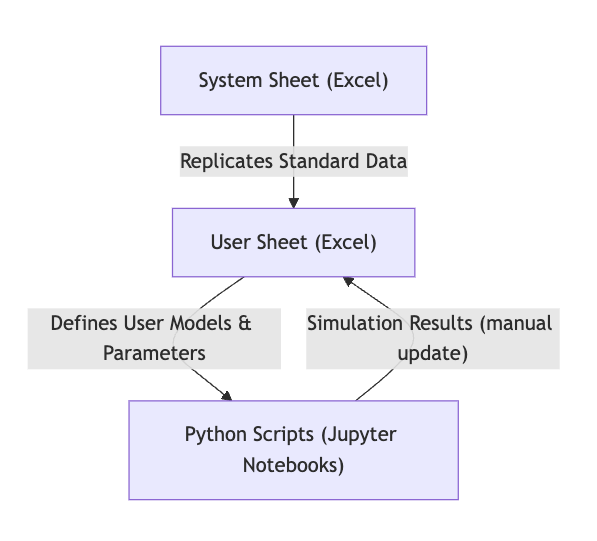
\includegraphics[scale=0.5]{./current_design}  
\end{center}

Important components are:
\begin{itemize}
    \item \textbf{User Sheet:}
    \begin{itemize}
        \item \textbf{Content:} Contains user-specific data, including customized plant models, parameters, and configurations.
        \item \textbf{Structure:} Over 30 workbooks detailing aspects like node parameters, stream properties, and operational constraints.
    \end{itemize}
    
    \item \textbf{System Sheet:}
    \begin{itemize}
        \item \textbf{Content:} Stores standardized industry data, default equipment parameters, and foundational models.
        \item \textbf{Structure:} Over 30 workbooks define templates for node models, ports, variables, and thermodynamic properties.
    \end{itemize}
    
    \item \textbf{Python Scripts:}
    \begin{itemize}
        \item \textbf{Environment:} Executed in Jupyter Notebooks.
        \item \textbf{Functionality:} Perform modeling and simulations based on data from Excel sheets.
        \item \textbf{Libraries used:} Python 3.8 with libraries such as NumPy, Pandas, and SciPy.
    \end{itemize}
    
    \item \textbf{Data Handling:}
    \begin{itemize}
        \item \textbf{Manual Processes:} Data is manually entered and updated in Excel. Parameters are manually referenced or exported for Python.
        \item \textbf{Simulation Workflow:} After data entry, Python scripts are manually run to perform simulations. Results are reviewed and documented externally.
    \end{itemize}

    
\end{itemize}
\subsection{Partner or Collaborative Applications}
\textbf{Existing Python-Based Mathematical Models:}\\\\
\textbf{Description}: Python scripts developed in Jupyter Notebooks by Dr. Mahalec’s team to perform complex mathematical modelling and simulations based on plant data.\\\\
\textbf{Software Interfaces}: The new software will interface with these scripts through a well-defined API or direct database connections, allowing seamless access to parameter data and the input/output of simulation results.

\subsection{Off-the-Shelf Software}
\noindent
\begin{tabularx}{\textwidth}{| X | X | X |}
    \hline
    \textbf{Product Name} & \textbf{Usage} & \textbf{Rationale} \\
    \hline
    ReactFlow & 
    ReactFlow will be used as a React-based library to manage the creation and manipulation of nodes and arcs within the graphical user interface (GUI). & 
    Dr. Mahalec advised using ReactFlow due to its features for handling complex node and arc interactions. It integrates with React, making development smoother, and has an active community that provides continuous support and updates.\\
    \hline
    dbgate & 
    dbgate will be used as the database management tool to provide users with a table-like interface for managing and editing data within the databases. & 
    Dr. Mahalec recommended dbgate for its versatility in handling both SQL and NoSQL database systems. It offers a user-friendly interface that simplifies data management tasks, allowing users to perform operations without needing specialized database training, making it an good choice for the project. \\
    \hline
\end{tabularx}
\subsection{Anticipated Workplace Environment}
The software will be used by individual users in a standard office setting, primarily on desktop or laptop computers. Users will access the web-based GUI through widely-used web browsers like Chrome, Firefox, or Edge. Each user may manage multiple plant models simultaneously, meaning the software must run smoothly on typical office hardware without requiring any specialized equipment. Since the office environment will have consistent internet access, this will support the web-based interface and ensure smooth integration with any necessary local systems.
\subsection{Schedule Constraints}
As stated in the SFWRENG 4G06 course outline, the schedule constraints are as follows:\\\\
\begin{table}[htbp!]
  \centering
  \begin{tabular}{|p{8cm}|p{3cm}|}
  \hline
  \textbf{Task} & \textbf{Date} \\ \hline
  Requirements Document Revision 0 & October 9 \\ \hline
  Hazard Analysis 0 & October 23 \\ \hline
  V\&V Plan Revision 0 & November 1 \\ \hline
  Proof of Concept Demonstration & November 11 to November 22 \\ \hline
  Design Document Revision 0 & January 15 \\ \hline
  Revision 0 Demonstration & February 3 to February 14 \\ \hline
  V\&V Report Revision 0 & March 7 \\ \hline
  Final Demonstration (Revision 1) & March 24 to March 30 \\ \hline
  EXPO Demonstration & April TBD \\ \hline
  Final Documentation (Revision 1) & April 2 \\ \hline
  \end{tabular}
  \caption{Project Timeline}
  \end{table}
  

\subsection{Budget Constraints}
This project will follow a zero-budget framework, relying entirely on free-tier and open-source software to minimize costs. All software components will run locally, avoiding any additional expenses apart from the purchase of ReactFlow Pro, which is required to access advanced node and arc examples as advised by Dr. Mahalec. If any purchases are necessary to meet the capstone deliverable requirements, the costs will be covered by the team members, with a total budget limit of \$750. Once the project is handed over to Dr. Mahalec, it will revert to operating under the zero-budget framework.
\subsection{Enterprise Constraints}
The software must operate entirely on local machines to comply with the enterprise’s data security and operational independence policies. This prohibits the use of external paid services and ensures that all data processing and storage are done within the organization’s internal infrastructure. Following these constraints guarantees the software maintains data integrity and aligns with enterprise standards for security and software usage.\\

Although the project will mostly use free-tier and open-source libraries, certain commercial components like ReactFlow Pro will be included to meet specific functional requirements. All components, whether commercial or open-source, must meet the organization’s compatibility and security standards, ensuring seamless integration within the local environment. This approach balances cost-efficiency with the use of specialized tools necessary for the project’s success.








\section{Naming Conventions and Terminology}
\subsection{Glossary of All Terms, Including Acronyms, Used by Stakeholders
involved in the Project}
\begin{itemize}
  \item UI: User Interface, refers to an interface that users can use to enter data inputs
  \item GUI: Graphical User Interface, refers to a user interface that includes graphics/images to reduce data complexity for theuser
  \item API: Application Programming Inteface: An abstracted programming layer that allows a user to interface with more complex systems without needing to have an understanding of the internals of that system
  \item: Node: Refers to a single machine in a factory
  \item: Edge: Refers to a connection between factory machines
  \item: Graph: Refers to a display that shows a series of nodes as shapes and a series of edges as arrows/lines
  \item Factory plant/plant: Refers to a factory building that is responsible for processing some sort of input into some sort of outputs through a series of nodes (factory machines) and edges (factory connections)
  \item Plant schema/schema: Refers to a graph shaped design for a factory plant via a series of nodes and edges on canvas
\end{itemize}


\section{Relevant Facts And Assumptions}
\subsection*{Relevant Facts}
\begin{itemize}
    
    \item The Python scripts simulate plant operations such as material flow and energy usage but currently require manual inputs and command-line execution.

    \item The final software, including code and documentation, will be owned by the client (Professor Mahalec) upon project completion, ensuring future use and modifications align with research objectives.

    \item Security measures, including NDAs and controlled data access, are in place to protect sensitive information and intellectual property throughout the project.
\end{itemize}

\subsection{Business Rules}
\begin{itemize}
    \item All simulation configurations, results, and user-generated data must be stored in a secure and accessible manner, with integrated services for future retrieval and analysis.
    \item The software should integrate seamlessly with existing Python models for plant simulations, ensuring accurate and efficient execution of simulations based on user inputs.
    \item The users want to use Business Intelligence tools outside of the application to analyze the output.
\end{itemize}              
\subsection{Assumptions}
\begin{itemize}
    \item The existing Python models are functional and will be provided by Dr. Mahalec’s team for integration into the new software solution.
    \item The project team has access to the necessary hardware and software resources required for development and testing, including the Python models.
    \item The project scope, as defined by the team and Professor Mahalec, will not change significantly during the course of development, barring any unforeseen technical challenges or new requirements from the client.
    \item It is assumed that Professor Mahalec will provide regular feedback and technical guidance to ensure the project stays aligned with research and educational goals.
    \item The software will primarily be used in an academic or research setting, and its potential deployment in an actual industrial environment would require further refinement and validation.
    \item The project will be developed using open-source tools and libraries, except where proprietary IP (e.g., the Python models) is used. Licensing for third-party tools will be managed in compliance with McMaster’s policies and relevant copyright laws. 
\end{itemize}

\section{The Scope of the Work}
\subsection{The Current Situation}
Currently, there exists a Python model that takes in data from a series of Excel tables, uses that data to simulate a plant and then outputs the results from that simulation. There is no UI or standardized method of entering the data nor is there a formal version control system that allows multiple users to save plant data and then recover it to continue working on it. Our solution produce a UI that would allow users to interface with the model without having the manually enter data while also providing a version control system that enables the user to save and recover work when needed. 
\subsection{The Context of the Work}
\begin{center}
  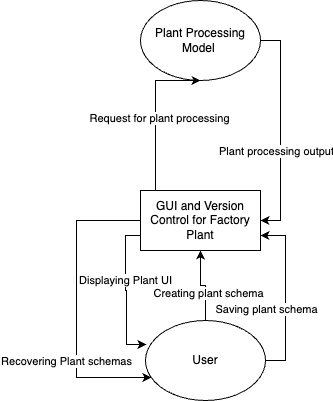
\includegraphics[scale=0.5]{./context_diagram}
\end{center}


In the above context diagram, we see the surrounding context of the system we are building. Our system is displayed by the square box in the center labeled GUI and version control for the factory plant with the two other nodes in the diagram representing external entities that our system needs to interact with. The arrows show the inputs/outputs of these different entities with the system. We can see that a user has various interactions with the system such as updating the schemas, saving schemas, and restoring previous schemas. The system in turn provides the user with a UI that allows them to visualize the plant as a response to these inputs. Similarly, our system interacts with an external Python model by sending it data and then receiving outputs from that data. 
\subsection{Work Partitioning}
\begin{tabularx}{\textwidth}{| X | X | X |}
  \hline
  \textbf{Event name} & \textbf{Input and Output} & \textbf{Summary of BUC} \\
  \hline
  Create factory node/edge & Create plant schema (in)
   & 
  A new node or edge is added by the user and displayed in the schema canvas\\
  \hline
  Delete factory node/edge & Create plant schema (in)
  & 
  The user deletes a given node/edge from the schema canvas \\
  \hline
  Move node/edge & Create plant schema (in)
  & 
  The user moves the position of a node or edge in the schema \\
  \hline
  Save schema & Saving plant schema (in)
  & 
  The user clicks to save a copy of the plant schema data \\
  \hline
  Restore schema & Recovering plant schema (in)
  & 
  The user clicks to restore/recover an existing saved schema \\
  \hline
  Display schema & Displaying plant UI (out)
  & 
  The system displays the current canvas to the user through the GUI \\
  \hline
  Send factory data & Request for plant processing (out)
  & 
  The system makes a request to the plant processing model containing the data of the factory inputs in order to get the factory outputs\\
  \hline
  Receive factory outputs & Plant processing output (in)
  & 
  The system receives the plant processing output data\\
  \hline
  
\end{tabularx}
\subsection{Specifying a Business Use Case (BUC)}
The specification for each business use case is detailed in the above table however a short summary below will provide more info. The business use cases can be summarized into four main types, user inputs, graphical output to user, request to model and response from model. The user inputs are when the user updates the schema, saves the schema and restores the schema and these are carried out via button press events in the system. The graphical output of the system is just the schema diagram displayed on a webpage for the user. The request to the model is an HTTP request carried out by the backend of our system to the model which lives in its own server. This request carries data in the form of an HTTP request body that contains the factory parameters. Finally, the response from the model is in the form of an HTTP response where in the response body we can find the output data of the factory. 

\section{Business Data Model and Data Dictionary}
\subsection{Business Data Model}
In the Class Diagram below User entity is main, representing everyone interacting with the system, from engineers to supervisors as mentioned in the stakeholders section. Each user can create multiple FactoryPlants, which represents different plant setups. Within each FactoryPlant, there are multiple Nodes and Edges. The Nodes represents different machines like reactors and pumps, each with its own set of parameters such as temperature and pressure. The Edges class, show the streams connecting these nodes, showcasing the flow of materials and info.
\\\\
Additionally, there is NodeType and EdgeType classes that classifies the different kind of Nodes and Edges available. For example, a NodeType defines a specific type of pump, while an EdgeType could specify whether a stream is gas or liquid. Each FactoryPlant/Map can undergo multiple Simulations, and each Simulation generates a SimulationResult, showing the results of the Python Script output ran by Dr. Mahalec's team. To keep track of changes and different versions of a FactoryPlant for different time period, there is also a Version class that allows users to look at different time period and change parameters for different period.
\\
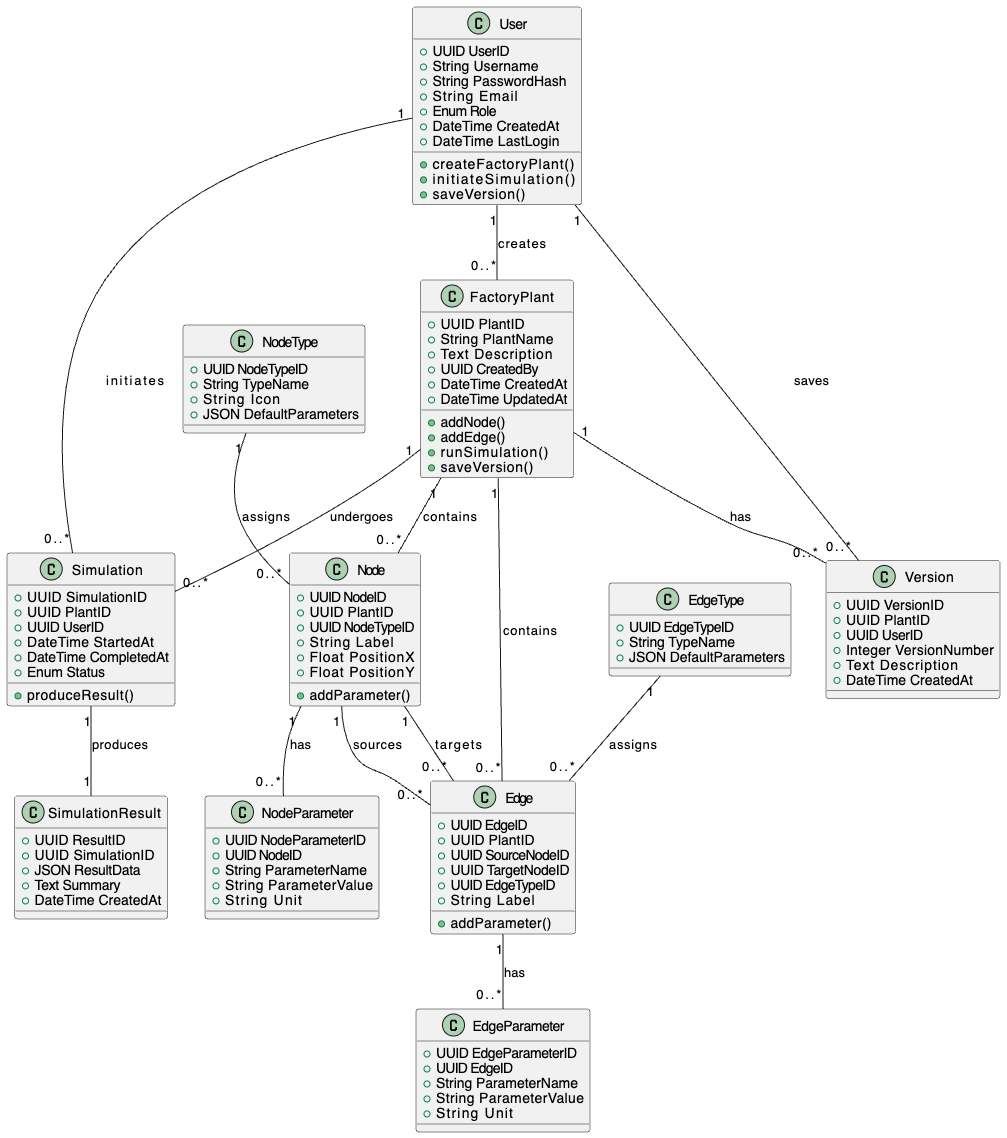
\includegraphics[scale=0.48]{./class_diagram}
\subsection{Data Dictionary}
\begin{longtable}{|p{3.5cm}|p{3.25cm}|p{2cm}|p{6cm}|}
  \hline
  \textbf{Class Name} & \textbf{Attribute Name} & \textbf{Data Type} & \textbf{Description} \\
  \hline
  \endfirsthead
  
  \hline
  \textbf{Class Name} & \textbf{Attribute Name} & \textbf{Data Type} & \textbf{Description} \\
  \hline
  \endhead
  
  % User Class
  \multirow{7}{*}{\textbf{User}} & UserID & UUID & Unique ID for each user \\
  \cline{2-4}
  & Username & String & The user’s login name \\
  \cline{2-4}
  & PasswordHash & String & Hashed password for auth \\
  \cline{2-4}
  & Email & String & User email address \\
  \cline{2-4}
  & Role & Enum & User roles eg: admin, user \\
  \cline{2-4}
  & CreatedAt & DateTime & Timestamp when account created \\
  \cline{2-4}
  & LastLogin & DateTime & Timestamp last user login \\
  \hline
  
  % FactoryPlant Class
  \multirow{6}{*}{\textbf{FactoryPlant}} & PlantID & UUID & Unique id for factory plant \\
  \cline{2-4}
  & PlantName & String & Name of the factory plant \\
  \cline{2-4}
  & Description & Text & Description of factory plant \\
  \cline{2-4}
  & CreatedBy & UUID (FK to User) & References the User who created the plant \\
  \cline{2-4}
  & CreatedAt & DateTime & Timestamp of when the plant was created \\
  \cline{2-4}
  & UpdatedAt & DateTime & Timestamp of when the plant was last updated \\
  \hline
  
  % Node (Machine) Class
  \multirow{6}{*}{\textbf{Node}} & NodeID & UUID & Unique id for each node \\
  \cline{2-4}
  & PlantID & UUID (FK to FactoryPlant) & Reference to the parent factory plant \\
  \cline{2-4}
  & NodeTypeID & UUID (FK to NodeType) & Reference to the type of node \\
  \cline{2-4}
  & Label & String & Display label for the node \\
  \cline{2-4}
  & PositionX & Float & X-coordinate position on the canvas \\
  \cline{2-4}
  & PositionY & Float & Y-coordinate position on the canvas \\
  \hline
  
  % Edge (Stream) Class
  \multirow{6}{*}{\textbf{Edge (Stream)}} & EdgeID & UUID & Unique id for each edge \\
  \cline{2-4}
  & PlantID & UUID (FK to FactoryPlant) & Reference to the parent factory plant \\
  \cline{2-4}
  & SourceNodeID & UUID (FK to Node) & Reference to the source node \\
  \cline{2-4}
  & TargetNodeID & UUID (FK to Node) & Reference to the target node \\
  \cline{2-4}
  & EdgeTypeID & UUID (FK to EdgeType) & Reference to the type of edge \\
  \cline{2-4}
  & Label & String & Display label for the edge \\
  \hline
  
  % NodeType Class
  \multirow{4}{*}{\textbf{NodeType}} & NodeTypeID & UUID & Unique id for each node type \\
  \cline{2-4}
  & TypeName & String & Name of the node type eg: Reactor, Pump \\
  \cline{2-4}
  & Icon & String & Icon representing the node (svg) \\
  \cline{2-4}
  & DefaultParameters & JSON & Default parameters for this node type \\
  \hline
  
  % EdgeType Class
  \multirow{3}{*}{\textbf{EdgeType}} & EdgeTypeID & UUID & Unique id for each edge type \\
  \cline{2-4}
  & TypeName & String & Name of the edge type eg: Gas Stream, Liquid Stream, etc \\
  \cline{2-4}
  & DefaultParameters & JSON & Default parameters for this edge type \\
  \hline
  
  % NodeParameter Class
  \multirow{5}{*}{\textbf{NodeParameter}} & NodeParameterID & UUID & Unique ID for each node parameter \\
  \cline{2-4}
  & NodeID & UUID (FK to Node) & Reference to the node \\
  \cline{2-4}
  & ParameterName & String & Name of the parameter eg: Temperature, Pressure, etc \\
  \cline{2-4}
  & ParameterValue & String/Float & Value of the parameter. \\
  \cline{2-4}
  & Unit & String & Unit of measurement eg: Celsius, Bar, etc \\
  \hline
  
  % EdgeParameter Class
  \multirow{5}{*}{\textbf{EdgeParameter}} & EdgeParameterID & UUID & Unique ID for each edge parameter \\
  \cline{2-4}
  & EdgeID & UUID (FK to Edge) & Reference to the edge \\
  \cline{2-4}
  & ParameterName & String & Name of the parameter eg: Flow Rate, Composition, etc \\
  \cline{2-4}
  & ParameterValue & String/Float & Value of the parameter \\
  \cline{2-4}
  & Unit & String & Unit of measurement eg: Liters per Minute \\
  \hline
  
  % Simulation Class
  \multirow{6}{*}{\textbf{Simulation}} & SimulationID & UUID & Unique ID for each simulation run \\
  \cline{2-4}
  & PlantID & UUID (FK to FactoryPlant) & Reference to the factory plant being simulated \\
  \cline{2-4}
  & UserID & UUID (FK to User) & Reference to the user who initiated the simulation \\
  \cline{2-4}
  & StartedAt & DateTime & Timestamp when the simulation started \\
  \cline{2-4}
  & CompletedAt & DateTime & Timestamp when the simulation completed \\
  \cline{2-4}
  & Status & Enum & Current status of the simulation eg: Pending, Running, Completed, Failed \\
  \hline
  
  % SimulationResult Class
  \multirow{5}{*}{\textbf{SimulationResult}} & ResultID & UUID & Unique ID for each simulation result \\
  \cline{2-4}
  & SimulationID & UUID (FK to Simulation) & Reference to the simulation\\
  \cline{2-4}
  & ResultData & JSON/Blob & Data output from the simulation \\
  \cline{2-4}
  & Summary & Text & Summary of the simulation results. \\
  \cline{2-4}
  & CreatedAt & DateTime & Timestamp when the result was created \\
  \hline
  
  % Version Class
  \multirow{6}{*}{\textbf{Version}} & VersionID & UUID & Unique ID for each version \\
  \cline{2-4}
  & PlantID & UUID (FK to FactoryPlant) & Reference to the factory plant associated with the version \\
  \cline{2-4}
  & UserID & UUID (FK to User) & Reference to the user who saved the version \\
  \cline{2-4}
  & VersionNumber & Integer &  Version number based on time period \\
  \cline{2-4}
  & Description & Text & Description \\
  \cline{2-4}
  & CreatedAt & DateTime & Timestamp when the version was saved \\
  \hline
\end{longtable}
  
\section{The Scope of the Product}

\subsection{Product Boundary}
The scope of the project includes the development of a software solution for modeling and simulating industrial plant operations. The software will consist of a graphical user interface (GUI) for building plant models, integrating with existing Python scripts through a backend server for simulating plant operations, and a database system for storing user configurations and simulation results. The product is being developed by Team 18 at McMaster University under the supervision of Professor Vladimir Mahalec. The goal is to improve the efficiency and accuracy of plant modeling while providing a user-friendly interface and robust backend capabilities.

The software will include the features and functionalities as defined in the requirements sections 9-17 of this document:

\subsection{Product Use Case Table}
The primary use cases of the software are outlined below:

\begin{table}[htbp!]
  \centering
  \begin{tabularx}{\textwidth}{|l|X|}
  \hline
  \textbf{Use Case ID} & \textbf{Description} \\ \hline
  UC-1 & \textbf{Create Plant Model}: Users can create a visual model of an industrial plant using the drag-and-drop GUI, adding nodes and edges to represent various processes and their interactions. \\ \hline
  UC-2 & \textbf{Run Plant Simulation}: Users can input data and run a simulation using the existing Python models. The simulation results will be displayed in the GUI. \\ \hline
  UC-3 & \textbf{Save and Load Plant Models}: Users can save their plant models to a local or remote database, and load existing models for modification or review. \\ \hline
  UC-4 & \textbf{View Simulation Results}: Simulation outputs, such as production rates, efficiency metrics, and potential bottlenecks, will be presented to users through the GUI. \\ \hline
  UC-5 & \textbf{Export Data}: Users can export simulation results and configuration data to external formats such as CSV or Excel for further analysis. \\ \hline
  UC-6 & \textbf{Manage User Accounts}: The software will support multi-user authentication, allowing different users to create and access their models securely. \\ \hline
  \end{tabularx}
  \caption{Product Use Case Table}
  \end{table}

\clearpage

\subsection{Individual Product Use Cases (PUC's)}
\begin{description}
    \item[PUC-1: Create Plant Model] \hfill \\
    The user opens the software and accesses the GUI, where they can drag and drop nodes onto a canvas to represent real components. Connections between nodes can be created using edges, establishing the relationships and workflows between different parts of the plant. Users can customize the properties of each node as defined in the system databases and save the configuration as a model.
    
    \item[PUC-2: Run Plant Simulation] \hfill \\
    After building a plant model, users can configure input parameters as defined in the system table as well as time periods for simulation. The system will use the existing Python models in the back end to perform computations and provide outputs in the GUI.

    \item[PUC-3: Save and Load Plant Models] \hfill \\
    Users can save the plant models into the database for later retrieval and modifications. Each saved model will include all node properties, connections, and configuration data, allowing users to resume their work or create different versions of the model.

    \item[PUC-4: View Simulation Results] \hfill \\
    The results of any simulation run are presented to the user in a relevant format within the GUI. 
    \item[PUC-5: Export Data] \hfill \\
    The system provides functionality to export simulation results and configuration data to common formats like CSV or Excel. This allows the user to leverage other Business Intelligence solutions to make better use of the data. 
 
    \item[PUC-6: Manage User Accounts] \hfill \\
    Users can create and manage individual accounts, which will allow for secure access to their saved plant models and simulation data. Multi-user authentication will ensure that data is protected and that different users can work on their own models independently.
\end{description}


\section{Functional Requirements}
\subsection{Functional Requirements}
\begin{tcolorbox}[title=FR1]
  \textbf{Description:} The product shall allow users to create and visually edit plant models by adding, deleting, or modifying nodes (representing machines) and edges (representing material streams). \\
  \textbf{Rationale:} Users need the ability to design complex industrial plants using a graphical interface to ensure accuracy and ease of use during the modeling process. \\
  \textbf{Fit Criterion:} A user can successfully add, delete, or modify nodes and edges in the plant model, and the changes are reflected in the graphical user interface.
  \end{tcolorbox}
  
  \vspace{0.5cm}
  
  \begin{tcolorbox}[title=FR2]
  \textbf{Description:} The product shall enable users to input variables and parameters for each machine and stream data for each edge before running simulations. \\
  \textbf{Rationale:} Accurate simulations require users to define specific operating conditions for machines (e.g., temperature, pressure) and material streams (e.g., flow rates, composition). \\
  \textbf{Fit Criterion:} Users are able to input variables for all nodes and edges, and the system successfully accepts and stores these inputs for use during simulations.
  \end{tcolorbox}
  
  \vspace{0.5cm}
  
  \begin{tcolorbox}[title=FR3]
  \textbf{Description:} The product shall integrate a custom solver to simulate the behavior of the plant model based on the input variables and parameters. \\
  \textbf{Rationale:} The system must be able to perform simulations to generate outputs that help users analyze and optimize the plant's performance. \\
  \textbf{Fit Criterion:} When the user runs a simulation, the product processes the model and input parameters, and produces a result based on the solver, which is viewable by the user.
  \end{tcolorbox}
  
  \vspace{0.5cm}
  
  \begin{tcolorbox}[title=FR4]
  \textbf{Description:} The product shall provide error messages when the model contains invalid or incomplete information (e.g., disconnected nodes or missing parameters). \\
  \textbf{Rationale:} To ensure accuracy, the system must notify users of errors before running a simulation, allowing them to correct the issues. \\
  \textbf{Fit Criterion:} When a user attempts to run a simulation with an incomplete or invalid model, the system displays a clear error message explaining the issue.
  \end{tcolorbox}
  
  \vspace{0.5cm}

\begin{tcolorbox}[title=FR5]
\textbf{Description:} The product shall allow users to save plant models locally in a standard file format. \\
\textbf{Rationale:} Users need the ability to save the current state of their model so that work can be resumed later or shared with others. \\
\textbf{Fit Criterion:} A user can save a plant model to a specified location, and the file contains all nodes, edges, and parameters for later use.
\end{tcolorbox}

\vspace{0.5cm}

\begin{tcolorbox}[title=FR6]
\textbf{Description:} The product shall allow users to load previously saved plant models from local storage. \\
\textbf{Rationale:} Users need to be able to reopen and edit plant models over multiple sessions. \\
\textbf{Fit Criterion:} A user can load a saved plant model from a file, and the application will restore all nodes, edges, and parameters as they were at the time of saving.
\end{tcolorbox}

\vspace{0.5cm}

\begin{tcolorbox}[title=FR7]
\textbf{Description:} The product shall support zooming and panning within the graphical user interface to allow users to view large or detailed plant models. \\
\textbf{Rationale:} Industrial plant models can become complex, and users need flexible navigation options to focus on different parts of the model. \\
\textbf{Fit Criterion:} Users can zoom in/out and pan across the model without losing visual fidelity or usability.
\end{tcolorbox}

\vspace{0.5cm}

\begin{tcolorbox}[title=FR8]
\textbf{Description:} The product shall allow users to export simulation results to a file format compatible with external analysis tools (e.g., CSV or Excel). \\
\textbf{Rationale:} Users may need to perform additional analysis on the simulation results outside the software. \\
\textbf{Fit Criterion:} After running a simulation, users can export the results to a CSV file for further analysis in tools like Excel or Python.
\end{tcolorbox}

\vspace{0.5cm}

\begin{tcolorbox}[title=FR9]
\textbf{Description:} The product shall validate input parameters before allowing the simulation to run. \\
\textbf{Rationale:} To avoid errors during the simulation, the system must ensure that all necessary input parameters are provided and valid. \\
\textbf{Fit Criterion:} If the user attempts to run a simulation with missing or invalid parameters, the system will display an error message and prevent the simulation from starting.
\end{tcolorbox}

\vspace{0.5cm}

\begin{tcolorbox}[title=FR10]
\textbf{Description:} The product shall provide real-time feedback as users modify the plant model, showing warnings if connections between nodes are missing or incorrect. \\
\textbf{Rationale:} This ensures that users are aware of potential issues as they build their model, preventing errors during simulation. \\
\textbf{Fit Criterion:} When a user creates or modifies nodes and edges, the system will highlight any invalid or incomplete connections in real-time.
\end{tcolorbox}


\section{Look and Feel Requirements}
\subsection{Appearance Requirements}
\begin{tcolorbox}[title=LAFAR1]
  \textbf{Description:} The product must feature a clear and logically structured layout that organizes information hierarchically to reflect the plant’s structure and process flow.
  
  \textbf{Rationale:} A structured layout will help users understand complex systems, making it easier to navigate and interact with the software during the modeling process.
  
  \textbf{Fit Criterion:} A user can successfully locate and navigate between different sections of the plant model without confusion, and information related to specific equipment and processes is presented in a clear, hierarchical manner.
\end{tcolorbox}

\vspace{0.5cm}

\begin{tcolorbox}[title=LAFAR2]
  \textbf{Description:} The product must use a consistent design across all elements, including fonts, colors, icons, and widgets, to ensure a cohesive and professional appearance.

  \textbf{Rationale:} Consistency in the design will reduce cognitive load and facilitate quicker recognition and interaction with the software components, enhancing user experience.

  \textbf{Fit Criterion:} All screens within the software should use the same font styles, color palette, iconography, and widget design, ensuring uniformity throughout the interface.
\end{tcolorbox}

\vspace{0.5cm}


\begin{tcolorbox}[title=LAFAR3]
  \textbf{Description:} The software must provide drag-and-drop functionality, allowing users to add, delete, or modify elements such as reactor, source, separator etc.

  \textbf{Rationale:} Drag-and-drop interactions simplify the process of constructing and modifying complex plant models, enhancing usability and reducing time required for model development.

  \textbf{Fit Criterion:} A user can successfully add, delete, or rearrange plant elements using drag-and-drop actions, and the changes are accurately reflected in the plant model.
\end{tcolorbox}

\subsection{Style Requirements}

\begin{tcolorbox}[title=LAFSR1]
  \textbf{Description:} The software must maintain sufficient contrast ratios between text, background colors, and interactive elements to ensure readability and accessibility.

  \textbf{Rationale:} Maintaining proper contrast ratios improves readability, making the software accessible to users with visual impairments and ensuring compliance with accessibility standards.

  \textbf{Fit Criterion:} All text and interactive elements must have a contrast ratio of at least 4.5:1 against their background colors as defined by WCAG (Web Content Accessibility Guidelines). The software must pass accessibility checks for color contrast.
\end{tcolorbox}
\vspace{0.5cm}
\begin{tcolorbox}[title=LAFSR2]
  \textbf{Description:} The software must utilize a neutral color scheme (e.g., grays, whites) with professional accent colors such as blue and green, reserved for emphasis and highlighting specific elements.

  \textbf{Rationale:} A neutral and professional color scheme maintains a clean and organized interface, minimizing visual distractions and allowing users to focus on the important aspects of the plant model.

  \textbf{Fit Criterion:} All screens and interface components must use a base color palette of neutral colors, with accent colors only used for actionable elements, alerts, or key information. No more than three accent colors should be present at any time.
\end{tcolorbox}

\vspace{0.5cm}

\begin{tcolorbox}[title=LAFSR3]
  \textbf{Description:} The software must incorporate clear visual cues, such as highlighting, shading, or outlines, to indicate interactivity and selectable elements.

  \textbf{Rationale:} Clear visual cues help users identify interactive elements such as buttons, input fields, and links, improving overall usability and navigation within the interface.

  \textbf{Fit Criterion:} All interactive elements, such as buttons and links, must change appearance (e.g., background color or border) when hovered over or selected, providing users with clear feedback on the element’s interactivity status.
\end{tcolorbox}

\vspace{0.5cm}

\section{Usability and Humanity Requirements}
\subsection{Ease of Use Requirements}
\begin{tcolorbox}[title=UHE1]
  \textbf{Description:} Each component of the service should be labeled with a descriptive tag that indicates what that component is used for \\
  \textbf{Rationale:} Since this is a GUI service, its important that the user is aware what different components of the interface are used for and to accomplish this we need clear labels \\
  \textbf{Fit Criterion:} Every component should have a one to one relationship with a clear label so that each UI component is well documented
\end{tcolorbox}
\begin{tcolorbox}[title=UHE2]
  \textbf{Description:} The UI control animations such as dragging and dropping nodes and edges should be smooth and without lag \\
  \textbf{Rationale:} A significant component of the UI is the animations that go into moving nodes and edges onto canvas. Its important these animations don't have lag that interrupt the users actions and so these animations should be lagless \\
  \textbf{Fit Criterion:} All animations should not buffer and should be verfied by third party reviews that the animations are smooth and seamless and easy to use 
\end{tcolorbox}
\subsection{Personalization and Internationalization Requirements}
\begin{tcolorbox}[title=UHPI1]
  \textbf{Description:} The system will use english everywhere throughout the system \\
  \textbf{Rationale:} The system will be used by english language speaking users and so it makes sense that the system is built with the english language\\
  \textbf{Fit Criterion:} Any text in the system will be written in english
\end{tcolorbox}
\subsection{Learning Requirements}
\begin{tcolorbox}[title=UHL1]
  \textbf{Description:} There should be documentation that enables a new user to learn the system \\
  \textbf{Rationale:} The system will be used by various new users and so it's important that new users are able to understand the system by following documentation\\
  \textbf{Fit Criterion:} When the system undergoes user testing, users should be able to learn and understand the system by following documentation within half an hour 
\end{tcolorbox}
\begin{tcolorbox}[title=UHL2]
  \textbf{Description:} There systems controls should be intuitive and easy to understand such that a new user can easily understand how to operate it\\
  \textbf{Rationale:} A schema designing software should take the complexity out of designing the schema to allow users to focus on design rather than operation of the software\\
  \textbf{Fit Criterion:} When the system undergoes user testing, new users should have no more than one question regarding how the controls of the system should be used
\end{tcolorbox}
\subsection{Understandability and Politeness Requirements}
\begin{tcolorbox}[title=UHU1]
  \textbf{Description:} The system will use language and terminology that can be understood by trained chemical engineers \\
  \textbf{Rationale:} The systems primary users will be educated chemical engineers and so the lanuage should be capable of being understood by educated chemical engineers\\
  \textbf{Fit Criterion:} Any chemical engineer with at least a bachelor's degree should be able to understand the terminology used in the system 
\end{tcolorbox}
\subsection{Accessibility Requirements}
\begin{tcolorbox}[title=UHA1]
  \textbf{Description:} The system can be used by any computer with a monitor, keyboard and mouse with all controls mapped to the keyboard and mouse \\
  \textbf{Rationale:} The system should be accessible by a standard engineer with a PC and so its important that all thats needed to operate it are basic computer peripherals like a  monitory keyboard and mouse. \\
  \textbf{Fit Criterion:} All of the systems outputs should be displayed by a monitor and all inputs can be handled by a keyboard and mouse. 
\end{tcolorbox}

\section{Performance Requirements}
\subsection{Speed and Latency Requirements}
\begin{tcolorbox}[title=PS1]
  \textbf{Description:} User inputs/interactions into the system should have a less than 60 ms latency \\
  \textbf{Rationale:} User inputs includ adding, moving and deleting nodes/edges from the canvas, these inputs should be quick and seamless so that the user can work without significant interruption and to make sure the system operates smoothly. \\
  \textbf{Fit Criterion:} All user interactions/inputs will have less than 60 ms latency from input to GUI output
\end{tcolorbox}
\begin{tcolorbox}[title=PS2]
  \textbf{Description:} Saving a schema to a filesystem should take less than 1 second \\
  \textbf{Rationale:} Saving a schema should not take a needlessly long amount of time and should be fast enough where a user can save multiple times without annoyance \\
  \textbf{Fit Criterion:} Saving a plant schema to the file system will have a maximum measured time of 1 second
\end{tcolorbox}
\begin{tcolorbox}[title=PS3]
  \textbf{Description:} Restoring a schema from the filesystem should take less than 1 second \\
  \textbf{Rationale:} Restoring a schema should not take a needlessly long amount of time and should be fast enough where a user can restore a schema painlessly \\
  \textbf{Fit Criterion:} Restoring a plant schema from the file system will have a maximum measured time of 1 second
\end{tcolorbox}
\begin{tcolorbox}[title=PS4]
  \textbf{Description:} Running the factory simulation model and getting outputs should take no longer than 10 seconds \\
  \textbf{Rationale:} While running the factory system model might take some time due to it being an external system, its important that making a request to this model and getting an output should not take too long which is why we are capping the maximum time to 10 seconds \\
  \textbf{Fit Criterion:} Running the model and getting an output will take a maximum measured time of 10 seconds. 
\end{tcolorbox}
\subsection{Safety-Critical Requirements}
This app does not require any safety-critical requirement since it's not a safety critical application. 
\subsection{Precision or Accuracy Requirements}
\begin{tcolorbox}[title=PPA1]
  \textbf{Description:} All numerical user inputs will not be constrained or rounded by the system \\
  \textbf{Rationale:} We do not want the system to apply its own assumptions on user inputs and so its important the system does not constrain user input and instead pass the numerical user input to the external processing model and let the model handle decisions regarding the input \\
  \textbf{Fit Criterion:} The system will not round or otherwise modify/constrain numerical user inputs 
\end{tcolorbox}
\begin{tcolorbox}[title=PPA2]
  \textbf{Description:} All graphical user inputs (creating/editing deleting nodes and edges) that are shown via the GUI will be sent to the model as whats shown in the canvas \\
  \textbf{Rationale:} Whatever the user sees on the canvas should match what the system sends to the model to avoid any misinterpretation between the system and the user \\
  \textbf{Fit Criterion:} The exact model shown on the canvas will represent the data that is sent to the processing model 
\end{tcolorbox}
\subsection{Robustness or Fault-Tolerance Requirements}
\begin{tcolorbox}[title=PRF1]
  \textbf{Description:} All failures or errors that the model produces will be displayed to the user with information regarding the error or failure \\
  \textbf{Rationale:} Errors and failures produced by the external processing model should not be hidden from the user, instead this information should be displayed to the user so that they can correct their inputs and try again \\
  \textbf{Fit Criterion:} If an error or failure is produced by the external model, a context box opens displaying information about the error/failure to the user
\end{tcolorbox}
\begin{tcolorbox}[title=PRF2]
  \textbf{Description:} All failures and errors from the system should be shown to the user with information regarding the error/failure \\
  \textbf{Rationale:} Errors and failures produced by the system should be shown to the user so that they can either fix their input or submit a bug request to get the problem fixed \\
  \textbf{Fit Criterion:} If the system results in an error or failure, a context box opens where the user is provided information regarding the error/failure
\end{tcolorbox}
\subsection{Capacity Requirements}
\begin{tcolorbox}[title=PC1]
  \textbf{Description:} The system should be able to handle schemas with utpo 100 nodes and 1000 edges \\
  \textbf{Rationale:} From the sample data, it appears that most schemas will have at most 100 nodes and 1000 edges so we can assume that this is the capacity limit for our schema \\
  \textbf{Fit Criterion:} The system will be constrained to handle 100 nodes and 1000 edges
\end{tcolorbox}
\subsection{Scalability or Extensibility Requirements}
\begin{tcolorbox}[title=PSE1]
  \textbf{Description:} The system should only need to be scalable to handle a single user \\
  \textbf{Rationale:} Since this system won't be used by multiple users at once, we only need the system to scale up to handle a single user \\
  \textbf{Fit Criterion:} The system will be stress tested such that it can handle the inputs from a single user
\end{tcolorbox}
\subsection{Longevity Requirements}
\begin{tcolorbox}[title=PL1]
  \textbf{Description:} The system should be maintainable without developer interference for at least 1 year\\
  \textbf{Rationale:} Since we are passing the system off to the sponsor after completion, it's important that the system can be maintained without developer support for a reasonable amount of time \\
  \textbf{Fit Criterion:} The system will be maintainable without developer support for at least 1 year
\end{tcolorbox}

\section{Operational and Environmental Requirements}

\subsection{Expected Physical Environment}

\begin{tcolorbox}[title=OEEP1]
\textbf{Description:} The product shall operate on standard web browsers such as Google Chrome, Mozilla Firefox, Microsoft Edge, and Safari, on both desktop and mobile devices. \\
\textbf{Rationale:} Users will likely access the web application from various browsers on different devices, so cross-browser compatibility is essential. \\
\textbf{Fit Criterion:} The web application functions seamlessly on the latest versions of Google Chrome, Firefox, Edge, and Safari, without browser-specific issues.
\end{tcolorbox}

\vspace{0.5cm}

\begin{tcolorbox}[title=OEEP2]
\textbf{Description:} The product shall be optimized for devices with a minimum of 4GB of RAM, and it shall function effectively on devices with at least a dual-core processor. \\
\textbf{Rationale:} Web applications are resource-light compared to desktop applications, but plant simulations may still be intensive. \\
\textbf{Fit Criterion:} The web application performs its core functions, including modeling and simulation, without excessive delays on devices meeting the minimum hardware requirements.
\end{tcolorbox}

\vspace{0.5cm}

\begin{tcolorbox}[title=OEEP3]
\textbf{Description:} The product shall provide a responsive interface, supporting screen resolutions from 1280x720 to 4K across different devices, including desktops, laptops, tablets, and smartphones. \\
\textbf{Rationale:} The web application needs to be accessible from a wide variety of devices and screen sizes. \\
\textbf{Fit Criterion:} The interface adapts to varying screen resolutions, providing a seamless user experience on both desktop and mobile devices without compromising usability.
\end{tcolorbox}

\vspace{0.5cm}

\subsection{Wider Environment Requirements}

\begin{tcolorbox}[title=OEWE1]
\textbf{Description:} The product shall require a continuous internet connection to perform all modeling, simulation, and collaboration tasks. \\
\textbf{Rationale:} The web application is designed to work online, and all features, including model creation, simulation, and saving, require an active internet connection to function. \\
\textbf{Fit Criterion:} The web application fails gracefully if the internet connection is lost, with appropriate error messages prompting users to reconnect.
\end{tcolorbox}

\vspace{0.5cm}

\begin{tcolorbox}[title=OEWE2]
\textbf{Description:} The product shall use a local MongoDB database hosted on the user’s server or local machine for all data storage. \\
\textbf{Rationale:} Users will maintain a local instance of MongoDB, ensuring that all data, including models and simulations, are stored and managed locally without reliance on external cloud services. \\
\textbf{Fit Criterion:} The web application successfully connects to the local MongoDB instance for data storage and retrieval, with no external cloud dependencies.
\end{tcolorbox}

\vspace{0.5cm}

\subsection{Requirements for Interfacing with Adjacent Systems}

\begin{tcolorbox}[title=OEIA1]
\textbf{Description:} The product shall allow users to export and import data using common formats such as CSV, Excel, and JSON to integrate with adjacent systems. \\
\textbf{Rationale:} Users need to transfer data between the web application and external tools for advanced analysis and reporting. \\
\textbf{Fit Criterion:} The web application allows users to export and import simulation data, model configurations, and results in CSV, Excel, or JSON formats.
\end{tcolorbox}

\vspace{0.5cm}

\begin{tcolorbox}[title=OEIA2]
\textbf{Description:} The product shall support API integration, enabling seamless data exchange with third-party tools such as simulation engines and enterprise resource planning (ERP) systems. \\
\textbf{Rationale:} Industrial users often work with various tools, so the web application must provide APIs to interact with other systems. \\
\textbf{Fit Criterion:} The application exposes RESTful APIs for data input and output, and it can communicate with external simulation engines or ERP systems without manual data transfers.
\end{tcolorbox}

\vspace{0.5cm}

\subsection{Productization Requirements}

\begin{tcolorbox}[title=OEP1]
\textbf{Description:} The product shall be distributed as a local executable that can be installed and run directly on a user's device without the need for additional server configurations. \\
\textbf{Rationale:} The product is intended to be used as a standalone application, accessible directly from the user's system without reliance on cloud infrastructure. \\
\textbf{Fit Criterion:} The product is available as an installer or a self-contained executable that users can download, install, and run on supported operating systems.
\end{tcolorbox}

\vspace{0.5cm}

\subsection{Release Requirements}

\begin{tcolorbox}[title=OER1]
\textbf{Description:} The product shall be released with full documentation, including an online help center, API documentation, and user guides. \\
\textbf{Rationale:} Comprehensive documentation is essential to assist users and developers in understanding and using the web application effectively. \\
\textbf{Fit Criterion:} The release includes an online help center, complete API documentation, and user guides accessible within the web application.
\end{tcolorbox}

\vspace{0.5cm}

\section{Maintainability and Support Requirements}

\subsection{Maintenance Requirements}

\begin{tcolorbox}[title=MSM1]
\textbf{Description:} All system maintenance must be completed at least one week prior to the release or any critical deployment. \\
\textbf{Rationale:} The product is being developed with key deadlines, and no updates should occur within one week of a major release to ensure a stable version for users. This reduces the risk of introducing bugs right before the system goes live. \\
\textbf{Fit Criterion:} No system updates, patches, or changes are made within one week of a critical release or deployment.
\end{tcolorbox}

\vspace{0.5cm}

\begin{tcolorbox}[title=MSM2]
\textbf{Description:} Maintenance tasks shall be logged and tracked using an issue management system such as GitHub Issues. \\
\textbf{Rationale:} Proper tracking of maintenance ensures that all issues are documented, prioritized, and resolved efficiently, reducing potential downtime and improving software quality. \\
\textbf{Fit Criterion:} All maintenance issues are logged, with at least 90\% of maintenance tasks tracked in the issue management system, and their status is visible to developers and users.
\end{tcolorbox}

\vspace{0.5cm}

\subsection{Supportability Requirements}

\begin{tcolorbox}[title=MSS1]
\textbf{Description:} Comprehensive technical documentation shall be provided, covering installation, configuration, usage, troubleshooting, and best practices for using the web application. \\
\textbf{Rationale:} Since the product may not be actively maintained after its release, clear and detailed documentation is essential for new users to be able to install, configure, and operate the system independently. \\
\textbf{Fit Criterion:} At least 80\% of users should report in a post-release survey that they can operate the system solely based on the provided documentation.
\end{tcolorbox}

\vspace{0.5cm}

\subsection{Adaptability Requirements}

\begin{tcolorbox}[title=MSA1]
\textbf{Description:} The system shall be modular, allowing future developers to add new features or make changes to the existing codebase with minimal effort. \\
\textbf{Rationale:} Although the initial product release may not require adaptability, future development may involve extending functionality or adapting to new requirements, so the codebase must support modularity and flexibility. \\
\textbf{Fit Criterion:} New modules or features can be integrated into the system without requiring major changes to the existing codebase, as verified by a developer inspection report.
\end{tcolorbox}

\vspace{0.5cm}

\begin{tcolorbox}[title=MSA2]
\textbf{Description:} The system shall be built using industry-standard tools and frameworks to ensure future developers can easily adapt and work on the project. \\
\textbf{Rationale:} Using widely recognized frameworks and tools will make the system more maintainable and adaptable, as future developers will not have to learn proprietary or uncommon technologies. \\
\textbf{Fit Criterion:} The system uses well-known and widely adopted technologies such as React, Node.js, and MongoDB, ensuring that new developers can quickly familiarize themselves with the project.
\end{tcolorbox}


\section{Security Requirements}

\subsection{Access Requirements}


\begin{tcolorbox}[title=SEC-ACC1]
\textbf{Description:} \textcolor{blue}{\sout{The system shall enforce role-based access control (RBAC) to restrict access to specific features and data based on user roles.}} \\
\textbf{Rationale:} \textcolor{blue}{\sout{RBAC ensures that users can only access information and perform actions that are relevant to their roles, minimizing security risks associated with excessive permissions.}} \\
\textbf{Fit Criterion:} \textcolor{blue}{\sout{The system defines roles such as Administrator, Operator, and Viewer, each with a distinct set of permissions and access rights.}}\\
\textbf{Explanation:}\textcolor{blue}{This requirement is being removed since our sponsor no longer requires us to have role based access control and so we do not need to consider this as a requirement within the scope of this project.}
\end{tcolorbox}

\subsection{Integrity Requirements}
\begin{tcolorbox}[title=SEC-INT1]
\textbf{Description:} The system shall ensure data integrity by validating and sanitizing all input fields. \\
\textbf{Rationale:} Validating and sanitizing inputs prevent malicious data from being processed by the system, reducing the risk of attacks such as SQL injection or XSS. \\
\textbf{Fit Criterion:} All inputs are validated against predefined formats, and inputs containing scripts or special characters are automatically sanitized or rejected.
\end{tcolorbox}

\begin{tcolorbox}[title=SEC-INT2]
\textbf{Description:} The system shall implement version control for configuration files and database entries to prevent unauthorized or untracked modifications. \\
\textbf{Rationale:} Version control helps maintain the integrity of configuration files and critical data by allowing the system to track changes and revert to previous states if needed. \\
\textbf{Fit Criterion:} The system uses a version control system (e.g., Git) for configuration files, and database entries are tracked using timestamps and unique identifiers.
\end{tcolorbox}

\subsection{Privacy Requirements}
\begin{tcolorbox}[title=SEC-PRI1]
\textbf{Description:} The system shall implement data encryption for sensitive user information both in transit and at rest. \\
\textbf{Rationale:} Encrypting sensitive data protects against unauthorized access and data breaches, ensuring compliance with privacy standards. \\
\textbf{Fit Criterion:} All sensitive data, such as user credentials and personal information, is encrypted using AES-256 at rest and SSL/TLS during transmission.
\end{tcolorbox}



\subsection{Audit Requirements}
\begin{tcolorbox}[title=SEC-AUD1]
\textbf{Description:} The system shall log all relevant user actions, including login attempts, data access, and modifications, for audit and monitoring purposes. \\
\textbf{Rationale:} Comprehensive logging helps in tracking user activities, detecting suspicious behavior, and conducting post-incident analysis. \\
\textbf{Fit Criterion:} The system records all user actions, including timestamps, user IDs, IP addresses, and the type of action, with logs stored securely and reviewed periodically.
\end{tcolorbox}



\subsection{Immunity Requirements}
\begin{tcolorbox}[title=SEC-IMM1]
\textbf{Description:} The system shall employ secure coding practices and automated security testing to detect and prevent vulnerabilities during development. \\
\textbf{Rationale:} Secure coding and testing reduce the likelihood of vulnerabilities being introduced into the system, enhancing its resilience against attacks. \\
\textbf{Fit Criterion:} The system undergoes automated security testing with tools like SAST (Static Application Security Testing) and DAST (Dynamic Application Security Testing) integrated into the development lifecycle.
\end{tcolorbox}



\section{Cultural Requirements}
\subsection{Cultural Requirements}
\begin{tcolorbox}[title=CR1]
  \textbf{Description:} The product shall be developed with consideration for the cultural practices and expectations of its users in an industrial setting, particularly in chemical plant operations. The primary language of the interface shall be English, and all symbols, colors, and terminology used in the product must be appropriate for professional use in business environments. \\
  \textbf{Rationale:} The product will be used in business settings like chemical factories, where clarity and cultural sensitivity are important to avoid misinterpretation. \\
  \textbf{Fit Criterion:} The system will undergo a review for every release to ensure that all symbols, colors, and terms are appropriate for use in industrial environments.
\end{tcolorbox}

\section{Compliance Requirements}
\subsection{Legal Requirements}
\begin{tcolorbox}[title=LR1]
  \textbf{Description:} The product shall comply with IP protection laws, with all IP developed (including code, database structures, and algorithms) being transferred to Dr. Mahalec under a proprietary license. The system must also adhere to data security laws to protect proprietary plant data and user information ensuring no data is leaked to unauthorized actor. \\
  \textbf{Rationale:} It is crucial to ensure proper IP protection because the product will be used in business settings that involve sensitive chemical plant operations. Compliance with data security laws ensures the confidentiality of user data and plant-specific information. \\
  \textbf{Fit Criterion:}  A legal review will be conducted at the end of the project when Dr. Mahalec purchases the software IP. This review will confirm the transfer of IP under a proprietary license and ensure compliance with data security laws. The documentation will confirm that no unauthorized access to the system’s information is possible, and this will be included in the final handover.
\end{tcolorbox}
\begin{tcolorbox}[title=LR2]
  \textbf{Description:} The system shall not use any copyrighted or patented technology without proper licensing or permission from the owner. This applies to third-party libraries, APIs, or external software integrated into the product. Any technology used must be appropriately licensed for commercial use and included in the final delivery. \\
  \textbf{Rationale:} The product will be using several third-party components during development. Ensuring that none of these components violate copyright or patent laws is important to prevent legal complications. \\
  \textbf{Fit Criterion:}  A review will be conducted by Dr. Malaec's legal team as well as by our capstone team to verify that no unlicensed or unauthorized technology (libraries or code) is used. All third-party software licenses will be documented, and necessary permissions will be secured.
\end{tcolorbox}
\subsection{Standards Compliance Requirements}
Discussed with Dr. Mahalec and team, currently the product that we are developing doesn’t need to be any specific industry or software standards compliant due to the internal nature of its use and the fact that it will be handed over for proprietary use within a controlled environment.

\section{Open Issues}

At this stage, the primary open issue concerns the selection of an Object-Relational Mapping (ORM) framework to effectively map data between the application and the databases. Given the architecture of our system, which involves both a SQL and NoSQL database, it's essential to choose an ORM that supports seamless integration with both database types or can be extended to support this functionality.

The decision on the ORM will affect several aspects of the project:
\begin{itemize}
    \item \textbf{Consistency and Maintainability}: A robust ORM will ensure that data is consistently managed between the frontend and backend, reducing the risk of mismatches or data corruption.
    \item \textbf{Performance}: The ORM choice will directly influence how efficiently the system can handle database operations, especially with large data sets and complex queries.
    \item \textbf{Flexibility}: The ORM should provide enough flexibility to allow for future database schema changes without significant refactoring of the codebase.
\end{itemize}

To address this issue, the team is currently evaluating several ORM frameworks, including those that offer multi-database support (e.g., for both SQL and NoSQL). Research is ongoing to determine which framework best suits the specific requirements of our system, taking into account factors such as:
\begin{itemize}
    \item Ease of use and integration
    \item Documentation and community support
    \item Performance with both types of databases
    \item Customization capabilities to handle specific data mapping needs
\end{itemize}

This decision is crucial as it will form the backbone of how data flows within the system, ensuring both scalability and reliability in future iterations of the product.

\section{Off-the-Shelf Solutions}

\subsection{Ready-Made Products}
Currently, there are no available products that can directly solve the unique challenges we are addressing. Our product is a custom solution aimed at modeling industrial plants using a node-and-edge-based system, combined with a simulation feature. Given the specificity of this domain and the custom simulation script provided by our sponsor, this will be the first of its kind.

However, while a complete solution does not exist, there are third-party tools that can assist in certain aspects of our project, particularly for the front-end and back-end development. These include:
\begin{itemize}
    \item ReactFlow (for node and edge management)
    \item ExpressJS (for building the back-end)
    \item PostgreSQL and MongoDB (for data management)
\end{itemize}

\subsection{Reusable Components}
Though the core functionality must be developed from scratch, we can leverage several reusable components to streamline specific areas of the project:
\begin{itemize}
    \item \textbf{ReactFlow:} This third-party library will manage the visual representation of nodes, edges, and the canvas in the front-end, making it easier to build and interact with the plant models.
    \item \textbf{PostgreSQL and MongoDB:} Widely used for managing system and user data, these databases will provide reliable, scalable data storage solutions.
    \item \textbf{Python Simulation Script:} Provided by our sponsor, this Python script will handle plant simulations, meaning no additional development is required for the core simulation logic.
\end{itemize}

\subsection{Products That Can Be Copied}
As our solution is designed to address a specific problem with no direct off-the-shelf equivalent, there are no complete products that can be copied or modified to meet our needs. However, we can draw inspiration from similar industrial modeling tools and best practices to inform the design of our system. Additionally, we will use and customize open-source libraries, such as ReactFlow, to meet our product’s unique requirements.

\section{New Problems}
\subsection{Effects on the Current Environment}
Rather than using Excel tables to interact with the python model, our system will enable the user to use a GUI to create the plant schemas which will then interact with the python model. This should be a seamless transition since the GUI will be simpler and more user friendly than the Excel tables and it should not cause any conflicts in the overall environment. 
\subsection{Effects on the Installed Systems}
The system will interface with the python model by making a request to an endpoint that will then process the input data via the python model. The endpoint will then respond to this request with the appropriate output data. 
\subsection{Potential User Problems}
Existing users will need to learn how to use the schema building tools. However this should not be too difficult as it just requires using a mouse and keyboard to drag, drop and modify nodes/edges which should be as simple or simpler than inputting the data manually through Excel. 
\subsection{Limitations in the Anticipated Implementation Environment That May
Inhibit the New Product}
We will need to customize our input data for the endpoint such that it fits with the specification of the Python model. This may require massaging and modifying the data so that the values stay consistent but the form fits the Python model which may be a difficult task. However we think that the changes to the shape of the data should not be too extreme and should be doable within the scope of the project. 
\subsection{Follow-Up Problems}
We will need to figure out how to create an efficient local deployment of the overall service in a way thats easy to setup for the user. This local deployment should be capable of spinning up a database, hosting an API server and building the client. 
\section{Tasks}
\subsection{Project Planning}
The project schedule will follow the deliverables deadlines outlined in the SFWRENG 4G06 course outline.\\ \\
\begin{table}[hbt!]
  \centering
  \begin{tabularx}{\textwidth}{|X|l|}
    \hline
    \textbf{Task} & \textbf{Date} \\ \hline
    Hazard Analysis 0 & October 23 \\ \hline
    V\&V Plan Revision 0 & November 1 \\ \hline
    Proof of Concept Demonstration & November 11 to November 22 \\ \hline
    Design Document Revision 0 & January 15 \\ \hline
    Revision 0 Demonstration & February 3 to February 14 \\ \hline
    V\&V Report Revision 0 & March 7 \\ \hline
    Final Demonstration (Revision 1) & March 24 to March 30 \\ \hline
    EXPO Demonstration & April TBD \\ \hline
    Final Documentation (Revision 1) & April 2 \\ \hline
  \end{tabularx}
  \caption{Project Timeline}
  \end{table}
\subsection{Planning of the Development Phases}
The development process will be divided into three major phases: GUI Development, Database and Schema Design, and Integration with Python Models. These phases will run in sequence, though some aspects of testing and integration will overlap as needed to ensure consistency throughout the project.

\subsubsection{Phase 1: GUI Development}
The primary goal of this phase is to create an intuitive, interactive interface that allows users to visualize and manipulate plant models.\\\\
In this phase, the team will first familiarize themselves with React Flow, which will be used to implement the node and edge creation features. The drag-and-drop functionality will be developed to enable users to place and organize components (nodes) on a canvas and connect them with arcs (edges). This system will serve as the foundation for building plant schemas within the software. Testing will ensure that the interface responds smoothly to user inputs and interactions, verifying that the canvas accurately represents the plant’s structure as users modify it.

\subsubsection{Phase 2: Database and Schema Design}
In this phase, the focus will be on designing a schema that stores network topology data, including nodes and arcs. This phase will involve setting up and structuring the databases, ensuring they are capable of storing user configurations, plant data, and model results.\\\\
The team will establish both SQL and NoSQL databases (PostgreSQL and MongoDB) to separate user-specific and system-specific data. Integrating these databases with the front-end will allow for real-time data flow between the user interface and the back-end, ensuring that changes made in the GUI are reflected in the database. This phase will also include rigorous testing to ensure data consistency and integrity as users interact with the interface.

\subsubsection{Phase 3: Integration with Python Models}
The final phase will focus on connecting the graphical interface with the existing Python simulation models provided by Dr. Mahalec. The Python models will simulate plant operations based on the input data provided through the GUI.\\\\
To achieve this, APIs will be developed to facilitate communication between the front-end and the Python models. Once integrated, the outputs of the simulations will be displayed in the GUI, providing users with visual feedback on the simulation results. Testing will ensure that data is correctly sent to and from the Python models, and that the simulations produce accurate outputs based on user input.

\section{Migration to the New Product}
\subsection{Requirements for Migration to the New Product}

The project team requires that all newly created databases and functionalities developed for the new system maintain backward compatibility with the existing models. This ensures that legacy functionalities continue to operate as expected without the need for significant modifications. Additionally, the new databases and functionalities should be designed with modularity and flexibility in mind, allowing them to be accessed, modified, and utilized independently of the graphical user interface (GUI) system. This enables external systems, scripts, or tools to interact with the database and leverage its capabilities, promoting greater interoperability and ease of integration for future development or enhancements.


\subsection{Data That Has to be Modified or Translated for the New System}

The current system heavily relies on a collection of unstructured Excel spreadsheets to store and manage crucial data. These spreadsheets contain not only the data and the variables but also mappings that support the execution of Python scripts used within the system. Due to the lack of structure and standardized data management practices, a significant amount of manual intervention is required to maintain and utilize these spreadsheets effectively. This manual processing poses challenges for efficiency, accuracy, and consistency.

To ensure a seamless transition to the new system, all critical data currently stored in these spreadsheets must be systematically restructured, translated, and integrated into the new database architecture. This will involve converting unstructured and disparate data into a cohesive format that aligns with the new system’s data models. Furthermore, the migration process must preserve the integrity and functionality of existing mappings and models, enabling the new system to interact with and utilize this data in an automated, streamlined manner without requiring additional manual intervention.
\section{Costs}
The only expense for the project so far is the price paid for React Flow Pro which is the pro version of the React Flow library which gives us access to sample React Flow components that we can integrate into our service. React Flow is a library that enables developers to build GUI that include node and edge diagram creation. The service costs \$195 in order to access the pro components which was paid by Dr. Mahelec. The other cost is time which is the 8 months of design and implementation time that we will need to fulfill the capstone. 
\section{User Documentation and Training}
\subsection{User Documentation Requirements}
The user documentation will provide important information for users interacting with the system. Since the system is closed source and will be used by a specific set of industry professionals, documentation will focus on the core functionalities. This includes:
\begin{itemize}
  \item A basic "Getting Started" guide included in the README file, providing an overview of system setup and usage.
  \item Step-by-step instructions for creating and modifying plant schemas using the GUI.
  \item Guidelines for managing and accessing plant models and user configurations within the database.
  \item A troubleshooting guide to resolve common issues related to database interactions or GUI operations.
\end{itemize}
\subsection{Training Requirements}
No formal training documentation is required. As the product is closed source and intended for use by Dr. Mahalec and his team, the system will be straightforward for them to operate with the provided documentation.

\section{Waiting Room}
If time permits we can try adding a live collaboration feature to the service such that multiple users can work on editing the canvas simultaneously. This would allow several users to work collaboratively on a project which would help improve its overall useability. However this is a feature that is not within the current scope of the project and is more of a bonus feature that can be completed if given extra time which is why it's in the waiting room. 

\section{Ideas for Solution}
\begin{itemize}
  \item The front-end of the product will be developed using React, a popular JavaScript library for building user interfaces. We plan to utilize ReactFlow, a third-party library, to manage the nodes, edges, and canvas interactions within the modeling environment.
  
  \item The back-end will be built using ExpressJS, a lightweight and efficient web framework for Node.js, which will handle server-side operations and API requests.
  
  \item For data storage, we will use PostgreSQL to manage system-related data and MongoDB to handle user-related data, ensuring scalability and flexibility in data management.
  
  \item The simulation engine will integrate a Python script provided by our sponsor, which will be responsible for calculating the simulated values based on user input and model configurations.
\end{itemize}


\newpage{}
\section*{Appendix --- Reflection}

The information in this section will be used to evaluate the team members on the
graduate attribute of Lifelong Learning.  Please answer the following questions:

\begin{enumerate}
  \item What knowledge and skills will the team collectively need to acquire to
  successfully complete this capstone project?  Examples of possible knowledge
  to acquire include domain specific knowledge from the domain of your
  application, or software engineering knowledge, mechatronics knowledge or
  computer science knowledge.  Skills may be related to technology, or writing,
  or presentation, or team management, etc.  You should look to identify at
  least one item for each team member.

  \textbf{Madhu:} I will need to learn how to write frontend react code using TypeScript, I will also need to learn how to use the react flow library to build diagram building software. \\\\
  \textbf{Dhrumil:} I need to learn how to manage two databases within the same system using a single ORM (Object-Relational Mapping) tool. This involves understanding how to handle both SQL and NoSQL databases in a unified way, ensuring that data flows smoothly between the GUI and the backend. Additionally, I need to learn TypeScript since our frontend will use it, and it is important for developing the React components that is in react flow.\\\\
  \textbf{Kishor:} I will be learning how to implement the databases locally and setting up the relations for the SQL database. \\\\
  \textbf{Rasik:} I will need to learn how to effectively translate ambiguous requirements into an effective GUI through consistent collaboration with stakeholders using react, react-flow, typescript and modelling tools\\\\
  \item For each of the knowledge areas and skills identified in the previous
  question, what are at least two approaches to acquiring the knowledge or
  mastering the skill?  Of the identified approaches, which will each team
  member pursue, and why did they make this choice? 
  
  \textbf{Madhu:} For learning TypeScript I can either try to follow virtual courses that help teach TypeScript which can be found on YouTube or try to reimplement an existing JavaScript using TypeScript which allows for experitiental learning. I will be looking at online courses since I find that I learn best by following a course. \\\\
  \textbf{Dhrumil:} To learn how to manage both SQL and NoSQL databases with a single ORM, I will look into official documentation of the db and the orm and do code-along activities that focus on implementing small scale project. I think that hands-on practice will help me better understand how to connect both types of databases within one system. For learning TypeScript, I will be using a YouTube tutorial, as I find video-based learning easy to follow. Code-along exercises will also help me pick up the language quickly.\\\\
  \textbf{Kishor: } For database implementation, I plan to use online resources, including official PostgreSQL and MongoDB documentation, along with tutorials that walk through the setup process and relational mapping. I may also reach out to my professor or classmates for additional guidance. I prefer learning through documentation and hands-on experience as it gives me the flexibility to try different configurations.\\\\
    \textbf{Rasik: } To effectively translate requirements into a functional system, I will deepen my understanding of industry best practices in UI development. I plan to leverage online resources, such as courses and professional forums, to enhance my knowledge of React and other relevant tools. I have a strong interest in collaborating with stakeholders to ensure that the team delivers solutions that precisely meet project requirements in an efficient and effective manner. I believe this skill is crucial, particularly for individuals aspiring to take on leadership roles in the future.  \\\\
\end{enumerate}

\end{document}
